
%  \section{The PSF profile analysis}

Since the 6-parameter PSF fits was adopted by the SDSS processing
pipeline, significant progress has been made in validating the von
Karman model of the atmosphere and measuring the associated outer
scale. See, for example, \cite{Tokovinin2002},
\cite{Boccas2004}, and \cite{MartinezMessenger}.
In this section, we describe our 2-parameter fits to the SDSS PSF
profiles using the von Karman atmosphere model.

Our fits to each PSF profile is a 2-step process. First we fit the
measured PSF profile to a von Karman PSF, with only one free parameter -
the FWHM of the von Karman profile. Although in most cases, the fitted
curve agrees with the input data points very well, better than the
original 6-parameter double-Gaussian fit, it doesn't always describe
the PSF tail beyond $\sim 15$ arcsec radius. This is obvious, because
it is known that the PSF tails in the optical bands can be quite
different due to the properties of the CCDs.
Therefore, in the second step of our PSF modeling, we introduce an
empirical instrument PSF, so that the observed PSF can be expressed as
a convolution of the atmosphere, represented by the von Karman, and
the instrument PSF,

\begin{equation}
        PSF = vK (FWHM) \otimes PSF_{inst},
\end{equation} 
where
\begin{equation}
        PSF_{inst} = \exp(-\frac{r^2}{2\sigma^2}) + 10^{\eta(ar^2+br+c)}.
\label{eq:psfinst}
\end{equation} 
Because the shape of the instrument PSF tail should not vary with
time, the parameters $a$, $b$, and $c$ in Eq.~(\ref{eq:psfinst}) are
fixed for each band-camera-column combination.
Even though this second fit involves a 2-dimensional convolution,
there is only one free parameter in the fit - 
$\eta$, the normalization of the instrument PSF tail.
Each two-step PSF fit can be done in a few seconds.

%o. keep 4 data points only
%o. not using r0 as parameter
%o. normalization to 1.
%o. give tailPar?


Why is SDSS PSF different for the $i$ band? The $i$ band psf has ``stronger tails''
becuse of scattering in the CCD.  The Si is transparent at long $i$-band wavelengths 
so light goes all the way through the chip and is reflected off the solder, and passes 
back up through the Si. This effect is not visible in the $z$ band because in this case
thick front-side chips are used (in all other bands, thin back-side chips are used). 

Compare to SDSS, emphasize superiority of 1 parameter vs. 6 parameters fit

Discuss profile shape stability when the seeing is rapidly  changing 

\begin{figure}
\centering
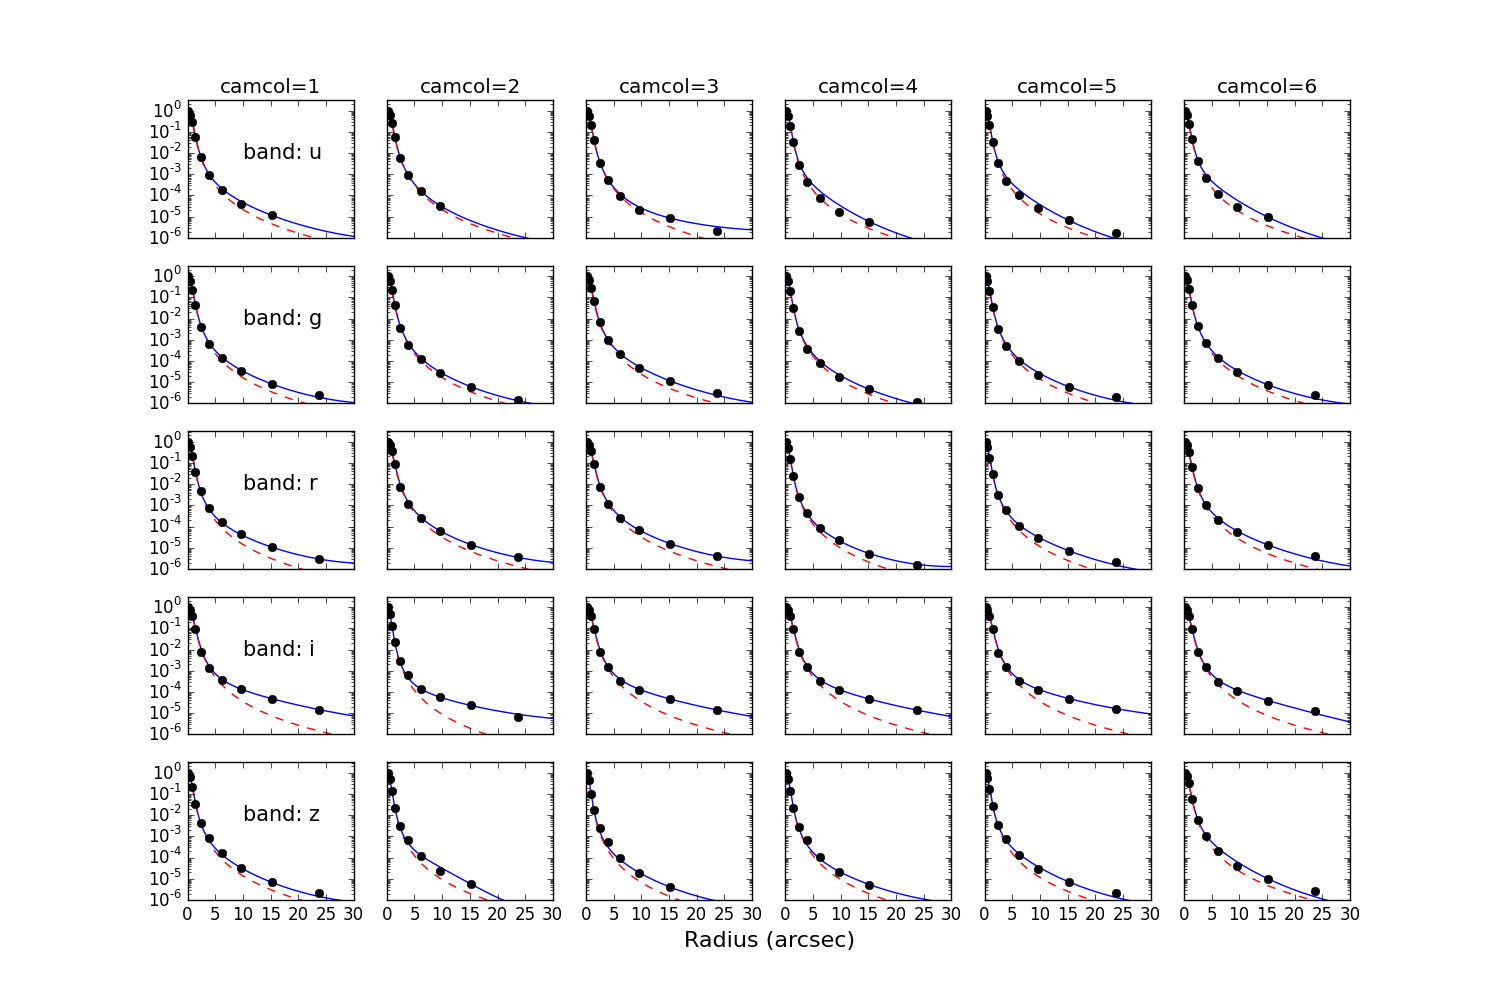
\includegraphics[width=0.9\textwidth]{FIGURES/psffit.png}
\caption{Fit to the PSF profiles from run 4874, field 0. Red curves
  are results of 1-parameter von Karman fits. Blue curves are red
  curve convolved with the instrument PSF, where the scaling factor on
  the tail component is allowed to vary. Note that the y-axis is on
  logorithm scale.
\label{fig:psffit}}
\end{figure}
